%%%%%%%%%%%%%%%%%%%%%%%%%%%%%%%%%%%%%%%%%
% Journal Article
% Database System
% Practical 10: Demonstrate any one concurrency scenario configuration and its impact on performance
%
% Gahan M. Saraiya
% 18MCEC10
%
%%%%%%%%%%%%%%%%%%%%%%%%%%%%%%%%%%%%%%%%%
%----------------------------------------------------------------------------------------
%       PACKAGES AND OTHER DOCUMENT CONFIGURATIONS
%----------------------------------------------------------------------------------------
\documentclass[paper=letter, fontsize=12pt]{article}
\usepackage[english]{babel} % English language/hyphenation
\usepackage{amsmath,amsfonts,amsthm} % Math packages
\usepackage[utf8]{inputenc}
\usepackage{xcolor}
\usepackage{float}
\usepackage{lipsum} % Package to generate dummy text throughout this template
\usepackage{blindtext}
\usepackage{graphicx} 
\usepackage{caption}
\usepackage{subcaption}
\usepackage[sc]{mathpazo} % Use the Palatino font
\usepackage[T1]{fontenc} % Use 8-bit encoding that has 256 glyphs
\usepackage{bbding}  % to use custom itemize font
\linespread{1.05} % Line spacing - Palatino needs more space between lines
\usepackage{microtype} % Slightly tweak font spacing for aesthetics
\usepackage[hmarginratio=1:1,top=32mm,columnsep=20pt]{geometry} % Document margins
\usepackage{multicol} % Used for the two-column layout of the document
%\usepackage[hang, small,labelfont=bf,up,textfont=it,up]{caption} % Custom captions under/above floats in tables or figures
\usepackage{booktabs} % Horizontal rules in tables
\usepackage{float} % Required for tables and figures in the multi-column environment - they need to be placed in specific locations with the [H] (e.g. \begin{table}[H])
\usepackage{hyperref} % For hyperlinks in the PDF
\usepackage{lettrine} % The lettrine is the first enlarged letter at the beginning of the text
\usepackage{paralist} % Used for the compactitem environment which makes bullet points with less space between them
\usepackage{abstract} % Allows abstract customization
\renewcommand{\abstractnamefont}{\normalfont\bfseries} % Set the "Abstract" text to bold
\renewcommand{\abstracttextfont}{\normalfont\small\itshape} % Set the abstract itself to small italic text
\usepackage{titlesec} % Allows customization of titles

\usepackage{makecell}
\usepackage{longtable}
\renewcommand\thesection{\Roman{section}} % Roman numerals for the sections
\renewcommand\thesubsection{\Roman{subsection}} % Roman numerals for subsections

\titleformat{\section}[block]{\large\scshape\centering}{\thesection.}{1em}{} % Change the look of the section titles
\titleformat{\subsection}[block]{\large}{\thesubsection.}{1em}{} % Change the look of the section titles
\newcommand{\horrule}[1]{\rule{\linewidth}{#1}} % Create horizontal rule command with 1 argument of height
\usepackage{fancyhdr} % Headers and footers
\pagestyle{fancy} % All pages have headers and footers
\fancyhead{} % Blank out the default header
\fancyfoot{} % Blank out the default footer

\fancyhead[C]{Institute of Technology, Nirma University $\bullet$ October 2018} % Custom header text

\fancyfoot[RO,LE]{\thepage} % Custom footer text
%----------------------------------------------------------------------------------------
%       TITLE SECTION
%----------------------------------------------------------------------------------------
\title{\vspace{-15mm}\fontsize{24pt}{10pt}\selectfont\textbf{Practical 10: Concurrency scenario configuration and its impact on performance}} % Article title
\author{
\large
{\textsc{Gahan Saraiya (18MCEC10), Rushi Trivedi(18MCEC08) }}\\[2mm]
%\thanks{A thank you or further information}\\ % Your name
\normalsize \href{mailto:18mcec10@nirmauni.ac.in}{18mcec10@nirmauni.ac.in, 18mcec08@nirmauni.ac.in}\\[2mm] % Your email address
}
\date{}
\hypersetup{
	colorlinks=true,
	linkcolor=blue,
	filecolor=magenta,      
	urlcolor=cyan,
	pdfauthor={Gahan Saraiya},
	pdfcreator={Gahan Saraiya},
	pdfproducer={Gahan Saraiya},
}
%----------------------------------------------------------------------------------------
\usepackage[utf8]{inputenc}
\usepackage[english]{babel}
\usepackage[utf8]{inputenc}
\usepackage{fourier} 
\usepackage{array}
\usepackage{makecell}

\renewcommand\theadalign{bc}
\renewcommand\theadfont{\bfseries}
\renewcommand\theadgape{\Gape[4pt]}
\renewcommand\cellgape{\Gape[4pt]}
\newcommand*\tick{\item[\Checkmark]}
\newcommand*\arrow{\item[$\Rightarrow$]}
\newcommand*\fail{\item[\XSolidBrush]}
\usepackage{minted} % for highlighting code sytax
\definecolor{LightGray}{gray}{0.9}

\setminted[text]{
	frame=lines, 
	breaklines,
	baselinestretch=1.2,
	bgcolor=LightGray,
%	fontsize=\small
}

\setminted[python]{
	frame=lines, 
	breaklines, 
	linenos,
	baselinestretch=1.2,
%	bgcolor=LightGray,
%	fontsize=\small
}

\begin{document}
\maketitle % Insert title
\thispagestyle{fancy} % All pages have headers and footers


\section{Introduction}
\paragraph{} Aim of this practical is to demonstrate any one concurrency scenario configuration and its impact on performance.

%\begin{table}
\renewcommand{\arraystretch}{2.5} % Default value: 1
\begin{longtable}{| c | p{12cm} |}
	\hline
	\multicolumn{2}{| c |}{\textbf{Table-level locks Available lock modes in PostgreSQL (used automatically; can also acquire explicitly)}}
	\\ \hline
	Lock & Context
	\\ \hline
	\hline
	ACCESS SHARE & The SELECT command acquires a lock of this mode on referenced tables. In general, any query that only reads a table and does not modify it will acquire this lock mode.
	\\
	ROW SHARE & The SELECT FOR UPDATE and SELECT FOR SHARE commands acquire a lock of this mode on the target table(s) (in addition to ACCESS SHARE locks on any other tables that are referenced but not selected FOR UPDATE/FOR SHARE).
	\\
	ROW EXCLUSIVE & The commands UPDATE, DELETE, and INSERT acquire this lock mode on the target table (in addition to ACCESS SHARE locks on any other referenced tables). In general, this lock mode will be acquired by any command that modifies data in a table.
	\\
	SHARE UPDATE EXCLUSIVE & Acquired by VACUUM (without FULL), ANALYZE, CREATE INDEX CONCURRENTLY, CREATE STATISTICS and ALTER TABLE VALIDATE and other ALTER TABLE variants (for full details see ALTER TABLE).
	\\
	SHARE & Acquired by CREATE INDEX (without CONCURRENTLY).
	\\
	SHARE ROW EXCLUSIVE & Acquired by CREATE COLLATION, CREATE TRIGGER, and many forms of ALTER TABLE (see ALTER TABLE).
	\\ 
	EXCLUSIVE & Acquired by REFRESH MATERIALIZED VIEW CONCURRENTLY.
	\\
	ACCESS EXCLUSIVE\footnote{Only an ACCESS EXCLUSIVE lock blocks a SELECT (without FOR UPDATE/SHARE) statement.} & Acquired by the DROP TABLE, TRUNCATE, REINDEX, CLUSTER, VACUUM FULL, and REFRESH MATERIALIZED VIEW (without CONCURRENTLY) commands. Many forms of ALTER TABLE also acquire a lock at this level. This is also the default lock mode for LOCK TABLE statements that do not specify a mode explicitly.
	\\ \hline
\end{longtable}
Once acquired, a lock is normally held till end of transaction. But if a lock is acquired after establishing a savepoint, the lock is released immediately if the savepoint is rolled back to. This is consistent with the principle that ROLLBACK cancels all effects of the commands since the savepoint. The same holds for locks acquired within a PL/pgSQL exception block: an error escape from the block releases locks acquired within it.

\section{Impact of Concurrency in PostgreSQL}
If running two queries concurrently using two separate connections at the same time in PostgreSQL --
\begin{itemize}
	\tick If they were both using sequential scans of the same table then in PostgreSQL it'd be a huge performance win because of its support for synchronized sequential scans.
	\tick If they shared the same indexes then they'd likely benefit from each others' reads in to cache.
	\fail If they're independent and touch different data then they might compete for I/O bandwidth, in which case they might take the same amount of time as running sequentially. If the I/O subsystem benefits from concurrency (higher net throughput with more clients) then the total time might be less. If the I/O subsystem handles concurrency poorly then they might take longer than running them sequentially. Or they might not be I/O bound at all, in which case if there's a free CPU for each they could well execute as if the other wasn't running at all.
\end{itemize}
Running 1,000 non-trivial queries concurrently --
\begin{itemize}
	\item PostgreSQL's own overheads in inter-process coordination, transaction and lock management, buffer management, etc. This can be quite a big cost, and PostgreSQL isn't really designed for high client counts
	\item Competition for working memory, cache, etc.
	\item Operating System scheduling overhead as it juggles 1000 competing processes all wanting time slices. Pretty minor these days, modern Operating Systems have fast schedulers.
	\item I/O thrashing. Most I/O systems have a peak performance client count. Sometimes it's 1, i.e. it's best with only one client, but it's often higher. Sometimes performance decreases again above the threshold. Sometimes it just reaches a plateau.
\end{itemize}

\pagebreak
\section{Summary}
\begin{figure}[h]
	\setlength{\parindent}{-10em} 
	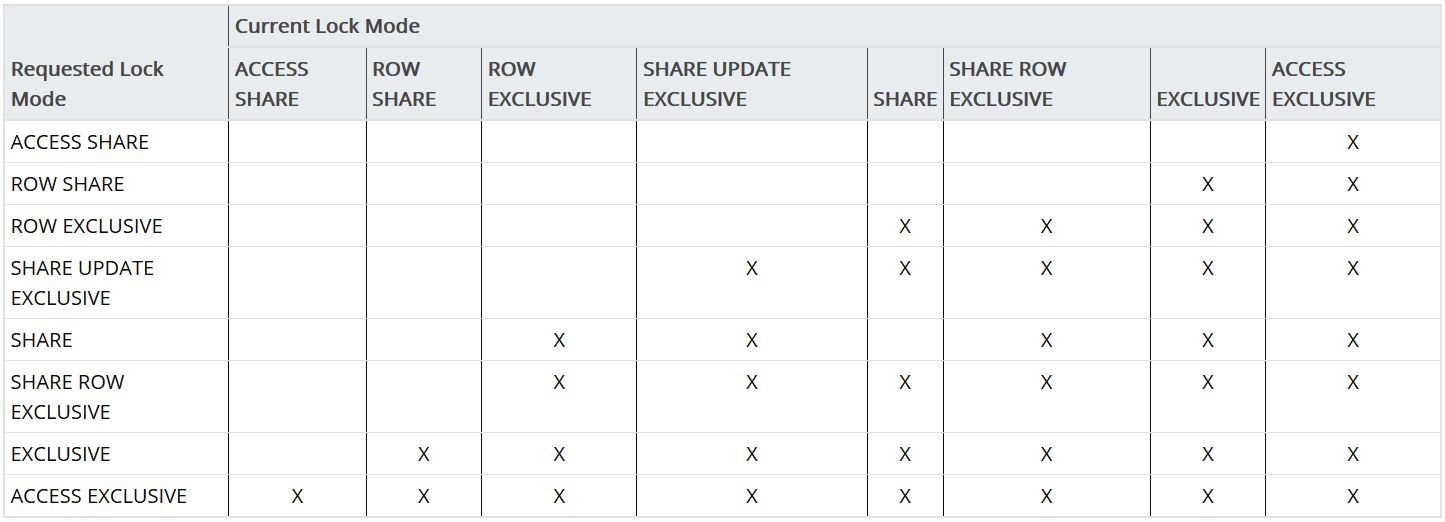
\includegraphics[width=600px]{assets/conflict-lock}
\end{figure}
PostgreSQL is an advanced RDBMS, with a solid foundation. The main service PostgreSQL implements to its users is a correct handling of concurrent operations. In the SQL model, that means handling both transactions and isolation levels.

A database server only has so many resources, and if you don't have enough connections active to use all of them, your throughput will generally improve by using more connections. Once all of the resources are in use, you won't push any more work through by having more connections competing for the resources. In fact, throughput starts to fall off due to the overhead from that contention. You can generally improve both latency and throughput by limiting the number of database connections with active transactions to match the available number of resources, and queuing any requests to start a new database transaction which come in while at the limit.

Contrary to many people's initial intuitive impulses, you will often see a transaction reach completion sooner if you queue it when it is ready but the system is busy enough to have saturated resources and start it later when resources become available. 


\end{document}
